%!TEX root = ../mbc_msc_thesis.tex

\chapter{Theoretical Framework}
\label{ch:theory}


\section{Introduction}

The main goal of this thesis project is to compare Bayesian methods in Deep Learning with traditional methods in the context of Active Learning. Traditional methods are based on the optimization of a loss function, which is rooted in maximum likelihood estimation and only offer a single point estimate with no measure of uncertainty in the prediction or the parameters, whereas the Bayesian approach gives a full posterior distribution for each of the parameters, thus giving as well as a posterior predictive distribution for the response variable. Bayesian methods avoid overfitting as they average over parameter values.

Bayesian methods for Artificial Neural Networks date back to the beginning of the 90s with Radford Neal's PhD thesis \cite{neal1996bayesian}, some work by \citeauthor{denker1991transforming} \cite{denker1991transforming} and \citeauthor{mackay1992practical} \cite{mackay1992practical}. In particular, \citeauthor{neal1996bayesian} basically used Hamiltonian Monte Carlo for posterior inferences of the parameters \cite{neal1996bayesian}. These approaches are not usually used because they are slow to train and do not scale well to the big networks and dataset used nowadays.

With the work of \citeauthor{gal2016uncertainty}, Bayesian approaches can be used for Deep Learning without making major changes to learning algorithms \cite{gal2016uncertainty}. In this work, this approach will be used and compared with traditional methods, particularly in the context of Active Learning, which aims to reduce the number of tagged examples for a supervised learning problem, as done in \cite{Gal2016Active}.

The reach and contributions of my thesis are to compare the Bayesian methods in Active Learning, such as extending the work of \cite{Gal2016Active} and do not retrain the whole model on each acquisition step, or try to find how many acquisition steps are necessary to get to the minimum error score gotten so far for a given architecture in the MNIST dataset. Or, as mentioned in \cite{gal2015bayesian}, it would be interesting to see if with less training examples from the ImageNet data and using Bayesian methods, we can achieve the same error rate that is achieved with the full dataset.



\section{Related work}

As mentioned before, Bayesian Artificial Neural Networks date back to late 1980s and early 1990s. These first approaches focused on Markov Chain Monte Carlo (MCMC) as the main method get samples of the posterior distribution of the parameters. Lately, there's been more work in the area, such as the Probabilistic Backpropagation algorithm developed by \citeauthor{hernandez2015probabilistic}, which relies on one-dimensional Gaussian distributions that approximate the marginal posterior distribution of the weights on each iteration of backpropagation \cite{hernandez2015probabilistic}. There is also the work by \citeauthor{graves2011practical}, based on variational inference to approximate the posterior distribution of the parameters \cite{graves2011practical}. These methods, however, do not scale well to very big network architectures and datasets; and they also have the disadvantage that they only work with multi-layer perceptron architectures, making them impossible to use with more recent architectures such as Convolutional Neural Networks (CNNs) or Recurrent Neural Networks (RNNs).

Recently, \citeauthor{gal2015dropout1} showed that a neural network with arbitrary depth, with dropout applied before each weight layer, is equivalent to the variational approximation to a deep Gaussian process. This is because the loss function minimizes the Kullback-Leibler divergence between an approximate distribution and the posterior of a deep Gaussian process \cite{gal2015dropout1}. This means that we can get uncertainty estimates with the models already trained with dropout without changing anything during training, the only difference comes at prediction time in which instead of doing a single forward pass and multiply each layer by a weight proportional to dropout probability, we just do several forward passes with dropout. They also showed in \cite{gal2015modern} that stochastic regularization techniques in arbitrary neural models can be seen as approximate variational inference in Bayesian Neural Networks.

This work is further extended by the same authors and they showed that the same ideas of dropout as a Bayesian approximation can be used in CNNs \cite{gal2015bayesian}. In particular, the showed that dropout can be seen as approximate variational inference in Bayesian Neural Networks, thus permitting the use of operations such as convolution and pooling in probabilistic models. The implementation is reduced to performing dropout after each convolution layer at training, and by performing several stochastic forward passes through the model (same idea as before). These stochastic forward passes are referred to as Monte Carlo (MC) dropout. Dropout is not usually performed after convolutional layers because it does not seem to give any benefits, but \citeauthor{gal2015bayesian} show empirically that MC-dropout can help with overfitting.

The work on CNNs is then used in an Active Learning environment, where the goal is to label images intelligently so that a model has good performance with a lower number of training examples \cite{Gal2016Active}. Deep learning poses several difficulties when used in an Active Learning setting because, first, small amounts of data need to be handled; and second, many Active Learning acquisition functions rely on model uncertainty, which is rarely represented in Deep Learning. \citeauthor{Gal2016Active} are able to achieve 5\% test error on the MNIST dataset with only 295 labeled images without, and 1.64\% test error with 1000 labeled images. They compare five different acquisition functions: choosing images that maximize the predictive entropy (Max Entropy); the ones that maximize the mutual information between predictions and model posterior (BALD); the ones that maximize the Variation Ratios; the ones that maximize mean standard deviation; and random acquisition (baseline). They also compare it with deterministic CNNs which, like the Bayesian CNN, produce a probability vector which can be used with the acquisition functions, but the Bayesian models, propagating uncertainty throughout the model, attain higher accuracy early on, and converge to a higher accuracy overall.

The dropout variational approach can also be used in Recurrent Neural Networks (RNNs), as shown by \citeauthor{gal2016theoretically} in \cite{gal2016theoretically}. In this paper, the authors give insight on how to use dropout with RNNs (something seldom done) and apply it on LSTM and GRU models, outperforming existing techniques in language modeling with the Penn Treebank dataset.

An example of how the uncertainties provided by Bayesian Neural Networks can be used, is shown by \citeauthor{li2017dropout} in \cite{li2017dropout}. They use adversarial examples and check if they can be told apart by examining the uncertainty representation of the dropout models. The deterministic Neural Networks produce over-confident predictions on these adversarial samples (they predict the wrong label very confidently), while dropout models, though producing wrong labels, are very uncertain about their predictions. They finish by stating that their results suggest that assessing the uncertainty of classification models can be used to identify adversarial examples, but much more research is needed to solve the difficulties faced with adversarial inputs.

The research on adversarial examples is continued by \citeauthor{rawat2017adversarial}, who study different Bayesian approaches (Bayes by Backprob (BBB), Probabilistic Backpropagation (PBP), Variational Matrix Gaussian (VMG) and MC-Dropout) and the uncertainty provided by the models, and prove that these models exhibit increased uncertainty when under attack \cite{rawat2017adversarial}. They state that all of the architectures in their study are Multi-Layer Perceptron, which do not scale for high dimensional colored images, with the exception of MC-Dropout, and therefore, a detailed study for MC-Dropout is required to demonstrate the applicability of model uncertainty for adversarial detection on various state-of-the-art attacks.


\section{Development}

The development so far has been to replicate \citeauthor{Gal2016Active}'s work done with MNIST dataset in \citetitle{Gal2016Active} and to implement two different architectures on a dataset provided by Amaury Gutiérrez that consists of pictures taken by drones before and after the September earthquake in three Mexican towns. Everything has been done in Keras using Tensorflow as backend and mainly through R, although some Python code was used via the \texttt{reticulate} package.

\subsection{Article replication}

My main goal in the replication  was to have an acquisition function that would outperform a random acquisition function. This was achieved and the results can be seen in figure \ref{fig:comparison_active_learning_random}, where one compare my results (on the left) with the original paper's results (right). The results are pretty similar overall, although the mean STD acquisition function was not implemented in the replication due to the bad performance shown in the paper.

Although my implementation achieved the goal of outperforming a random acquisition function, when comparing Bayesian and frequentist approaches the results differ. The paper's authors claim that the use of a Bayesian approach in the acquisition process of Active Learning leads to better accuracy with fewer images, but in my implementation there is virtually no distinction between both approaches. This can be seen in figures in \ref{fig:pred_entropy_AL} and \ref{fig:var_ratios_AL} that show my results (left) and the paper's authors results (right). In the paper, the frequentist acquisition functions show a worse performance than their Bayesian counterparts, but in my implementation there is no distinction. For example, with predictive entropy in figure \ref{fig:pred_entropy_AL}, the frequentist acquisition function in the original paper achieve a 90\% accuracy with around 300 images, while in my implementation this accuracy is first achieved with around 200 images.

%
% \begin{figure}[H]
%     \centering
%     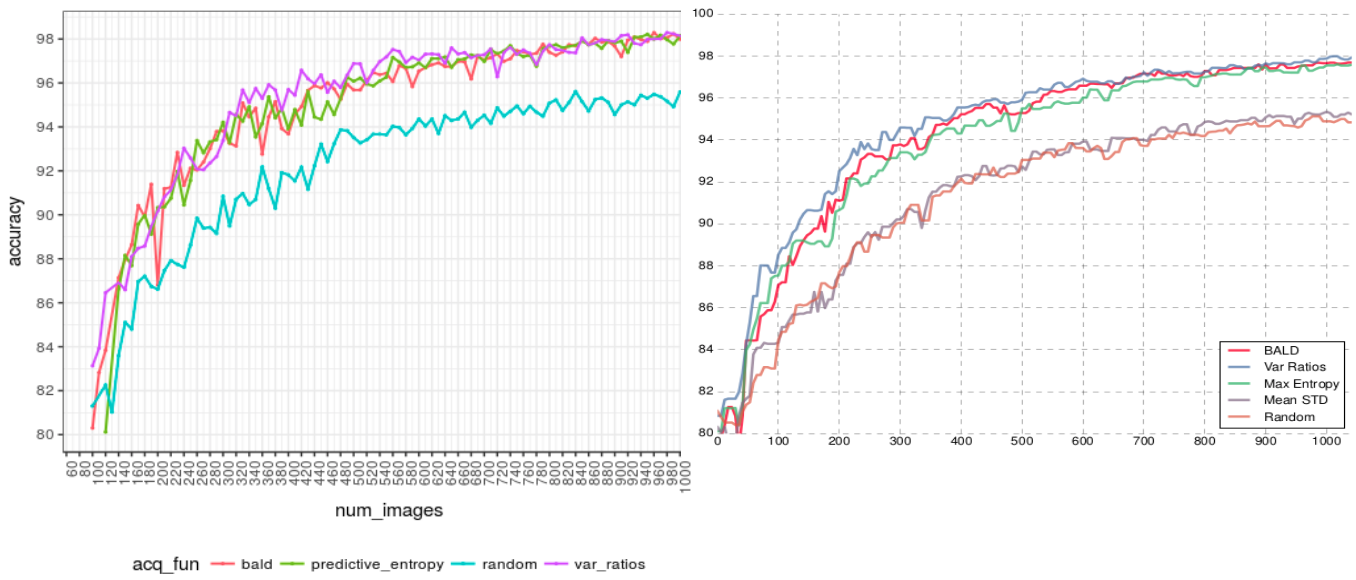
\includegraphics[width=\textwidth]{img_01.png}
%     \caption{Accuracy of models in each acquisition step. The left picture shows my implementation and the right picture shows \citeauthor{Gal2016Active}'s implementation.}
%     \label{fig:comparison_active_learning_random}
% \end{figure}
%
% \begin{figure}[H]
%   \centering
%   \subfloat[My results.]{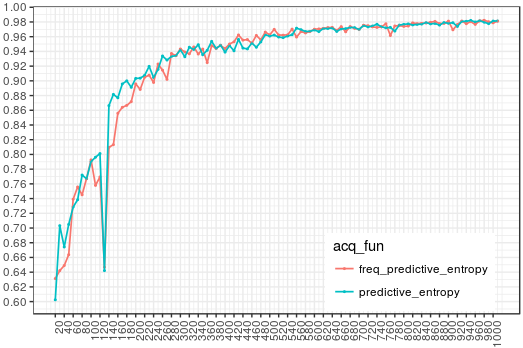
\includegraphics[width=0.5\textwidth]{pred_entropy_mine.png}}
%   \hfill
%   \subfloat[Paper's results.]{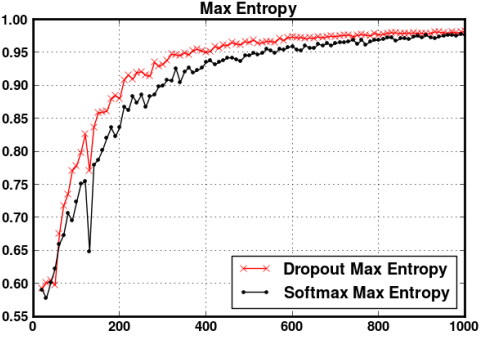
\includegraphics[width=0.5\textwidth]{pred_entropy_islam.png}}
%   \caption{Accuracy of Bayesian and frequentist models in each acquisition step using predictive entropy as acquisition function. The left picture shows my implementation and the right picture shows \citeauthor{Gal2016Active}'s implementation.}
%   \label{fig:pred_entropy_AL}
% \end{figure}
%
%
% \begin{figure}[H]
%   \centering
%   \subfloat[My results.]{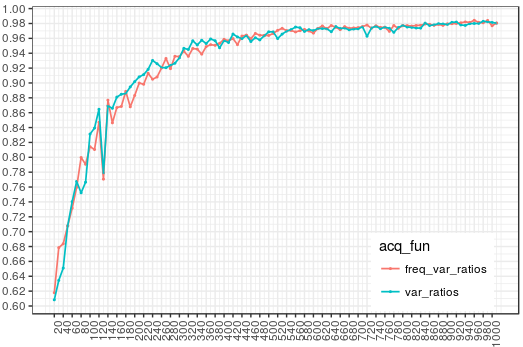
\includegraphics[width=0.5\textwidth]{var_ratio_mine.png}}
%   \hfill
%   \subfloat[Paper's results.]{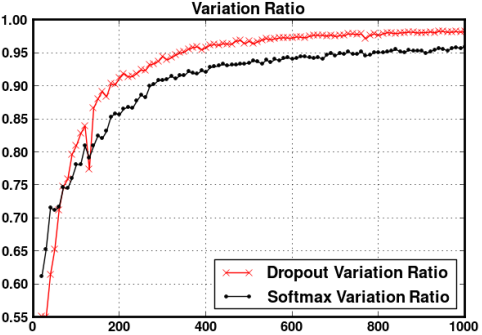
\includegraphics[width=0.5\textwidth]{var_ratio_islam.png}}
%   \caption{Accuracy of Bayesian and frequentist models in each acquisition step using variation ratios as acquisition function. The left picture shows my implementation and the right picture shows \citeauthor{Gal2016Active}'s implementation.}
%   \label{fig:var_ratios_AL}
% \end{figure}

One more thing that should be mentioned is that I could not implement the BALD acquisition in the frequentist setting because of the way it is defined. The BALD uncertainty for a prediction $y$ given model parameters $\mathcal{W}$, features $x$ and training data $\mathcal{D}$ is defined as

\begin{equation}
	\label{eq:bald_def}
	\mathbb{I}[y, \mathcal{W} | x, \mathcal{D}] = \mathbb{H}[y | x, \mathcal{D}] - \mathbb{E}_{p(\mathcal{W} | \mathcal{D})}[\mathbb{H}[y | x, \mathcal{W}]]
\end{equation}

with $\mathbb{H}[y | x, \mathcal{D}]$ is the predictive entropy and is defined as $-\sum_c p(y = c | x, \mathcal{D}) \log p(y = c | x, \mathcal{D})$. In the Bayesian case, we have a set of $T$ dropout samples that approximate the predictive distribution, so the second part of equation \ref{eq:bald_def}, i.e., the expected value $\mathbb{E}_{p(\mathcal{W} | \mathcal{D})}[\mathbb{H}[y | x, \mathcal{W}]]$ is approximated by averaging the predictive entropy of each predictive sample; this way $\mathbb{I}[y, \mathcal{W} | x, \mathcal{D}]$ is computed by taking the difference of this quantity and the first part of equation \ref{eq:bald_def}. In the frequentist case, we only have one point estimate, so that difference is zero, so $\mathbb{I}[y, \mathcal{W} | x, \mathcal{D}]$ is zero for all points in the pool set. To this day, I don't know how the paper's authors computed it because their Github code is not clear and they haven't answered my email where I asked them that.
